% ============================================================
%  chapters/proposal_body.tex —— 开题报告正文（官方表格 4 节结构）
%
%  内容源：thesis/proposal.md（由本文件经 scripts/tex2md.py 生成的可编辑镜像）
%  v3（2026-11-03）按任务书 v6 与导师意见改写：
%    1. 删去一.1 的“课题基本信息”表（封面已含，任务书 v6 亦不再单列）；
%    2. 一.2 由“国内外研究现状和发展趋势”改为“文献综述”，按五条脉络重排，
%       原一.1 的智能体能力文献移入综述第（一）节，正文引用顺序保持 [1]—[44]；
%    3. 二.2 改为“初步实施方案”，按理论研究、数据模型、算法方法、原型功能、
%       评估验证五个模块作学术化论述，删去四层架构、风险表、人日工作量、
%       可行性清单等软工报告式内容；进度表按任务书 v6 的 6 阶段教学周重排。
%
%  图表编号：由 \tjformsecnum{n} 按一级小节号接管（图 2-1、表 2-1 …）；
%  正文交叉引用一律 \ref，不写旧稿的图 6-1 / 表 10-1 等编号。
%
%  摘要块：官方开题报告表格无“摘要”栏；本课题保留原稿摘要以便与 Word 版对照，
%  由 \iftjproposalabstract 开关控制（定义于 chapters/tj-extras.tex）。
%  学院若不允许摘要，删除下面 \iftjproposalabstract … \fi 之间的内容即可
%  （开关本身保留，不影响编译）。
% ============================================================

% ---- PDF 链接锚点：\tjformsecnum 重定义了 \thetable/\thefigure，但 hyperref 的
% \theHtable/\theHfigure 仍按 chapter 计数（无 chapter 时恒为 0.1），图表共用同一
% 锚点，xdvipdfmx 因此报 "Object @table.0.1 already defined"。让 H 锚点跟随显示编号。
\makeatletter
\renewcommand{\theHtable}{\thetable}
\renewcommand{\theHfigure}{\thefigure}
\makeatother

\iftjproposalabstract
\tjformsection{摘要}

开发者借助代码智能体完成代码修改、执行与测试已成为常态，但对话、变更、工具调用与测试结果分散在不同界面，缺少以开发任务为中心的组织，使“为何这样修改、依据什么验证、中断后如何接续”难以回答。本课题面向单个开发者，研究任务、对话、变更、工具调用与测试之间的关联与组织方法，设计并实现支持任务上下文追踪与变更溯源的 Web 原型，并从概念与模型、采集与关联、溯源与续接、评估四个方面提出初步实施方案。本研究定位为小样本探索性预研，结论以 6—8 个任务与 4—5 名受试者的描述统计结果表述。

\textbf{关键词}：代码智能体；任务上下文；变更溯源；中断恢复；证据链
\fi

\tjformsection{一、\tjheadertext 课题背景}\tjformsecnum{1}

\tjformsubsection{1．课题来源及研究的目的和意义}

近年来，代码智能体（code agent）逐渐应用于日常软件开发。开发者以自然语言描述任务，由智能体完成代码分析、文件修改、工具调用、测试执行与问题排查。与代码补全不同，智能体的产出并非一段建议代码，而是一组带有工具调用与执行反馈的操作序列；开发过程由此从“人写代码”转变为“人下指令、智能体实施、人审查验证”的协作过程。这一转变在提高任务吞吐的同时，也使“过程是否可理解、可核查、可接续”成为开发者必须面对的问题。

然而，现有工具通常将过程信息分散于不同界面或不同类型的记录之中：对话留存于会话窗口，代码差异留存于 diff 视图，工具调用留存于终端日志，测试结果留存于测试报告，版本演化留存于 Git 历史。这些记录之间既缺少共同标识，也缺少以开发任务为中心的组织。由此产生三方面问题：一是任务视角缺失，在多轮修改、多任务并行与中断重启后难以掌握当前进展；二是溯源断裂，代码因何而改、依据哪次测试验证，只能依靠人工查找与回忆；三是上下文丢失，重新开始工作时需重读长对话与大量差异。

本课题面向单个开发者使用代码智能体完成开发任务的场景，研究开发任务、对话、代码变更、工具调用与测试结果之间的关联与组织方法，设计并实现支持任务上下文追踪与变更溯源的 Web 原型，使开发者能够围绕任务、文件或代码片段审视“为何修改、依据何在、验证结果如何”，并在任务中断后恢复必要的上下文。

本课题的意义体现在三个层面。理论层面，将“任务上下文”与“变更溯源”的概念从 IDE 与桌面场景迁移至智能体驱动的“指令—工具调用—变更—测试”序列，建立其与 PROV 的映射，并讨论任务边界判定、异构记录关联与证据充分性等表示问题。实践层面，将关联、溯源与恢复实现为可查询、可复现的原型，为单个开发者提供可操作的证据链，而非停留于日志浏览。教学层面，完整经历“问题识别—文献定位—模型设计—原型实现—实证评估”的研究流程，并明确说明小样本评估结论的适用边界。

\tjformsubsection{2．文献综述}

本节按“代码智能体与软件工程自动化—变更分析与代码历史—任务上下文与中断恢复—过程溯源与证据链—工程工具现状”五条脉络梳理相关研究，依次回答智能体能力如何评价、改了什么、过程围绕什么组织、依据什么证明，以及在工程实践中落地如何。检索以 Google Scholar、DBLP、arXiv、ACM Digital Library 与《软件学报》为主，检索词含 code agent、task context、provenance、resumption 等，覆盖 2004—2026 年的 40 篇（条）文献与文档，其中中文期刊论文 2 篇、标准与产品文档 6 条；检索式与命中数待定稿阶段补充。

\tjformsubsub{（一）代码智能体与软件工程自动化}

能力评价取决于任务与判据的设定。面向真实仓库的评测以 SWE-bench 为代表：按含问题描述、含测试改动、新增测试可转为通过等条件过滤，保留 2,294 个可判定实例，以 FAIL_TO_PASS 与 PASS_TO_PASS 为判据，测试补丁单独提供以免模型改动判据[1]；当时最佳模型仅解决 1.96\% 的任务[1]。更早的评测以函数级、单轮任务为主：HumanEval 以文档串生成函数体、按功能正确性判定，报告模型解决 28.8\% 的问题[2]，其口径便于比较，但粒度较窄。

此后工作沿三条路径改进。在接口与执行环境上，SWE-agent 主张能力受限于模型与计算机之间的接口，设计搜索、查看、编辑等命令并约束返回规模，使 SWE-bench Lite 通过率由检索增强基线的 1.31\% 升至 18.0\%，全量测试集为 12.47\%[3]；OpenHands 把智能体状态建模为事件流，动作、观察与成本均以事件记录，在 15 个基准上评测，Lite 通过率 26.0\%[4]。在动作表示上，CodeAct 将动作统一为可执行 Python 代码，中间结果留在解释器、仅回传打印输出与异常，最高提升 20 个百分点、17 题中 12 题最优[5]。在流程组织上，MetaGPT 把标准流程编码为五个角色的提示序列，返工次数由 2.5 降至 0.83[6]；ChatDev 以三阶段对话链组织两个角色，生成程序可执行性为 0.88[7]。但据 OpenHands 的评测，Agentless 以更简化的流程取得 27.3\% 的 Lite 通过率，高于 OpenHands 的 26.0\%[4,8]。

已有综述总结了软件工程全流程的进展[9-10]，中文文献中另有检索增强综述[11]与故障复现测试生成工作[12]。能力提升并未消除使用代价，但证据多以最终结果为口径：一项对照实验在单一任务（JavaScript 实现 HTTP 服务器）上报告 Copilot 使完成速度提升 55.8\%，任务单一，不宜外推[13]；行为研究显示验证与理解生成代码占用可观时间[14]，AI 助手用户写出代码的安全性更低且更自信[15]，人机交互可分加速型与探索型[16]，期望与体验存在落差[17]。这些研究考察的仍是最终产物与主观体验；而智能体的指令、工具调用、变更与测试构成操作序列，哪条指令触发修改、哪次测试完成验证，不在评价口径之内。这正是本课题的出发点之一：产出若要被信任与接续，须伴随可核查的过程证据。

\tjformsubsub{（二）变更分析与代码历史}

相邻的脉络关注代码变更本身。SZZ 以修复提交引用的缺陷报告为线索，回溯引入缺陷的那次变更，在提交层面把“修复”与“引入”联系起来[18]。一项综述厘清了该脉络的粒度边界：Kagdi 等按“演化对象—研究目的—表示方式—信息来源”四层梳理仓库挖掘，指出多数工作以文件或行号为表示单位、以提交与缺陷库为信息来源[19]；据该综述转述，已有研究在 433,833 条修改中把 23,540 条关联到缺陷报告；变更预测任务上，基于元数据的最好精确率（基于文件）与召回率（基于历史）分别为 12\% 与 87\%；“修复又引发后续修复”的事务规模平均为 3.82，修复诱导的事务约为非修复诱导事务的 3 倍[19]。仅凭提交与缺陷库的元数据难以支撑可靠的变更关联，变更须先界定单位，这正是本课题以变更块（hunk）为溯源单位的动因。Robbes 与 Lanza 主张以变更为中心刻画软件演化[20]。

表示粒度亦在细化：GumTree 以抽象语法树匹配生成细于行级的编辑脚本[21]，CodeShovel 重建方法级代码历史[22]。这些工作使“改了什么”的刻画日益精确，但关联对象始终是提交与仓库实体，变更的触发来源与验证依据不在其表示范围内；而智能体场景中的变更与过程事件同处一个会话过程，提交级粒度难以承载这种时序关系。

\tjformsubsub{（三）任务上下文与中断恢复}

以任务为单位组织上下文并非新命题。Mylyn 提出任务上下文模型，按所选任务与近期活动过滤 IDE 代码元素[23]；TaskTracer 在桌面环境中把文件、邮件与网页归集到正在处理的任务[24]；ActivitySpace 跨应用推荐与当前任务相关的代码元素[25]；Codebook 建立代码实体与提交、缺陷报告、邮件之间的关联图[26]。前三者表明任务可作为聚合信息的入口，Codebook 则说明代码实体可与仓库记录关联；但线索来源为 IDE 元素、窗口事件与仓库元数据，均不涉及智能体的指令与工具调用。

中断恢复研究为“上下文应包含什么”提供了实证依据。Parnin 与 Rugaber 结合 86 名开发者的 9,899 个会话日志与 414 份问卷，发现自报的上下文丢失程度比日志所示高出 2—10 倍；该文以 15 分钟空闲切分会话（属分析假设而非结论，会话亦不等同于任务），并报告恢复线索中即时差异、变更摘要与代码缩略图的偏好得分依次为 3.9、3.4 与 3.2[27]。该排序支持本课题以变更及其差异为恢复入口的取舍。Parnin 与 DeLine 以受控实验比较情景线索与语义线索[28]，Safer 与 Murphy 比较两类任务边界识别界面[29]，Robbes 与 Lanza 刻画了开发会话的结构[30]。

上述工作的共同前提是：任务由开发者显式声明或由界面界定，线索来自编辑与窗口事件，恢复目标是回到原工作状态。而智能体场景中任务多以自然语言指令提出，未被显式声明，线索由指令文本、工具调用参数与执行输出构成，开发者还需确认此前的修改是否有依据。任务上下文因此须扩展到“指令—工具调用—变更—测试”序列，恢复对象亦应从编辑位置扩展为带证据的进展。

\tjformsubsub{（四）过程溯源与证据链}

回答“依据什么”需要溯源方法支撑。数据库领域把溯源（provenance）抽象为为什么、如何、在何处三类问题[31]；PROV-O 将溯源对象抽象为实体、活动与代理三类，并已成为跨系统交换的溯源标准[32]；PROV-AGENT 把溯源扩展至提示、响应与决策等交互要素，使一轮智能体交互可被记录为溯源单元[33]。Whyline 以“为什么”式提问组织执行证据[34]；noWorkflow 把脚本执行捕获为溯源图，以内容寻址标识（SHA1）作为外键、以一次执行（trial）为版本单位支持差异比较、状态恢复与历史查询，并可沿数据依赖回溯取值来源[35]。

上述工作确立了证据链的基本形态，但用于智能体开发过程仍有三处不适配：溯源实体是数据或脚本状态而非代码变更，缺少与文件、变更块及行号对应的变更单位；验证依据（测试运行与结果）未进入溯源图，无法回答“这次修改依据哪次测试”；PROV-AGENT 虽覆盖提示、响应与决策，但面向交互元数据，未与代码变更建立派生关系。本课题的信息模型因此需在 PROV-O 框架上补充变更块与验证依据两类节点及其与任务、消息、工具调用的边。

\tjformsubsub{（五）工程工具现状与研究述评}

客户端与可观测性工具可视为上述研究的产业侧近似实现。Claude Code 通过钩子与 stream-json 事件流暴露会话过程，会话记录以 JSONL 存于用户目录的项目文件夹，文档给出存储位置与恢复方式，但未提供格式的版本化契约与兼容性承诺[36]；Cursor 的命令行接口同样支持 stream-json 输出[37]；Cline 以影子 Git 仓库记录快照，在每次工具调用后提交当前文件状态，使任务内检查点可恢复[38]。可观测性一侧，Langfuse 提供模型调用的可观测性与追踪[39]；OpenTelemetry 则发布生成式 AI 语义约定，该规范已迁至独立仓库维护[40]。

将上述脉络与工程工具并置，前述任务视角、溯源与上下文问题可归为三处空缺。组织单位上，任务上下文研究以显式任务为根，智能体研究以数据集任务或扁平事件流为单位，缺少“由开发者提出、可跨会话延续”的任务层[3-4,23]。变更粒度上，仓库挖掘与代码历史以文件、行或方法为单位，客户端以快照或检查点为单位，均未达到可与证据绑定的变更块级[18-19,21-22,36-38]。验证依据上，就所检材料看，测试在智能体研究中主要作为评测判据，在 IDE 场景研究中基本不涉及，“某次修改依据哪次测试”缺少可查询的表示[1,3,27-29]。对照见表~\ref{tab:compare}；该表仅列代表性工作，“未涉及”指所查材料中未见相应设计，而非原作者明确排除。

\begin{table}[H]
  \centering
  \caption{代表性工作的组织单位与证据覆盖}
  \label{tab:compare}
  \setlength{\tabcolsep}{4pt}
  \begin{tabularx}{\linewidth}{@{}>{\raggedright\arraybackslash}p{3.3cm}>{\raggedright\arraybackslash}p{2.9cm}>{\raggedright\arraybackslash}p{2.6cm}>{\raggedright\arraybackslash}p{2.4cm}>{\raggedright\arraybackslash}X@{}}
    \toprule
    代表性工作 & 组织单位 & 变更或记录粒度 & 验证依据 & 智能体事件流 \\
    \midrule
    Mylyn[23] & 显式任务 & IDE 代码元素 & 未涉及 & 否 \\
    Codebook[26] & 仓库实体 & 实体、提交 & 未涉及 & 否 \\
    noWorkflow[35] & 一次执行（trial） & 变量赋值 & 未涉及 & 否 \\
    PROV-AGENT[33] & 工作流 & 提示、响应 & 摘要未涉及 & 是 \\
    SWE-agent[3] & 单次任务（实例） & 编辑、命令 & 仅评测判据 & 是 \\
    客户端[36-38] & 会话、文件 & 快照与检查点 & 未涉及 & 是 \\
    本课题 & 开发任务 & 变更块 & 测试运行 & 是 \\
    \bottomrule
  \end{tabularx}
\end{table}

本课题的切入点可概括为三点：以开发任务为根节点统一关联对话、变更、工具调用与测试；使变更粒度达到变更块并支持“代码—原因—证据”双向查询；把测试运行与结果纳入证据链，使“某次修改依据哪次测试”可查询。大语言模型摘要与进展整理在此基础上以证据绑定约束，证据不足时弃答；三点效果由评估模块检验。“以任务为单位组织上下文”本身并非空白：Mylyn[23] 与恢复研究[27-28] 已提供模型与实证基础，本课题的差异在于研究对象从人在 IDE 中的编辑事件转为智能体驱动的“指令—工具调用—变更—测试”序列，并把验证依据纳入证据链。上述判断限于所检文献与文档（截至 2026 年 10 月），定稿阶段将补充系统检索，以免以“未见”代“不存在”。

\tjformsection{二、\tjheadertext 方案介绍}\tjformsecnum{2}

\tjformsubsection{1．研究问题与研究内容}

本课题关注的核心问题是：单个开发者使用代码智能体完成开发任务时，如何将分散于对话、变更、工具调用与测试记录中的过程信息组织起来，使之可追溯、可核查，并在任务中断后支持上下文恢复。该问题包含三个相互关联的方面：一是采用何种信息模型统一表示异构记录，使任务、对话、变更、执行与测试之间能够建立稳定关联；二是依据哪些线索将上述记录归并到具体任务，并判定任务的起止边界；三是如何围绕代码变更组织证据、呈现任务进展，并在中断后恢复必要的上下文。三者分别对应表示、关联与恢复三个层面，评估则贯穿其中。研究方法上，拟采用文献分析、模型设计、原型实现与实证评估相结合的方式，先建立表示与关联方法，再通过原型检验其可用性。

围绕上述问题，本课题的研究内容主要包括五个方面。一是任务上下文的信息模型与统一事件表示，抽象开发任务、对话轮次、消息、工具调用、文件变更、测试运行、测试用例结果与检查点等实体及其关系，设计可扩展的事件模式，使不同来源的记录进入同一表示框架。二是上下文采集与关联，接入代码智能体的会话与工具调用、文件系统与 Git、测试报告，将编辑动作归一化为变更块，并利用时间邻近、显式引用与文件级位置映射等线索建立变更与对话之间的多对多关联。三是变更溯源与证据链，以变更块为单位记录触发来源、实施过程、修改前后快照、验证依据与后续演化，支持从代码到原因、从原因到代码的双向查询。四是交互界面与任务续接，设计任务中心、任务时间线与变更证据侧栏等视图，并在任务中断后生成任务快照，呈现已完成、未完成与待验证事项。五是大语言模型辅助与评估，在证据绑定约束下生成任务摘要与进展整理，并通过典型编程任务考察系统在代码理解、修改原因分析与任务衔接方面的作用。

\tjformsubsection{2．初步实施方案}

本课题的初步实施方案按“概念与模型—采集与关联—溯源与续接—评估”四个模块组织。四个模块对应研究推进的不同环节：概念与模型回答“表示什么”，采集与关联回答“如何获得并建立联系”，溯源与续接回答“如何查询与使用”，评估回答“方案是否有效”。四者并非软件工程的层次划分，而是相互约束的研究环节，其关系如图~\ref{fig:route} 所示。

\begin{figure}[H]
  \centering
  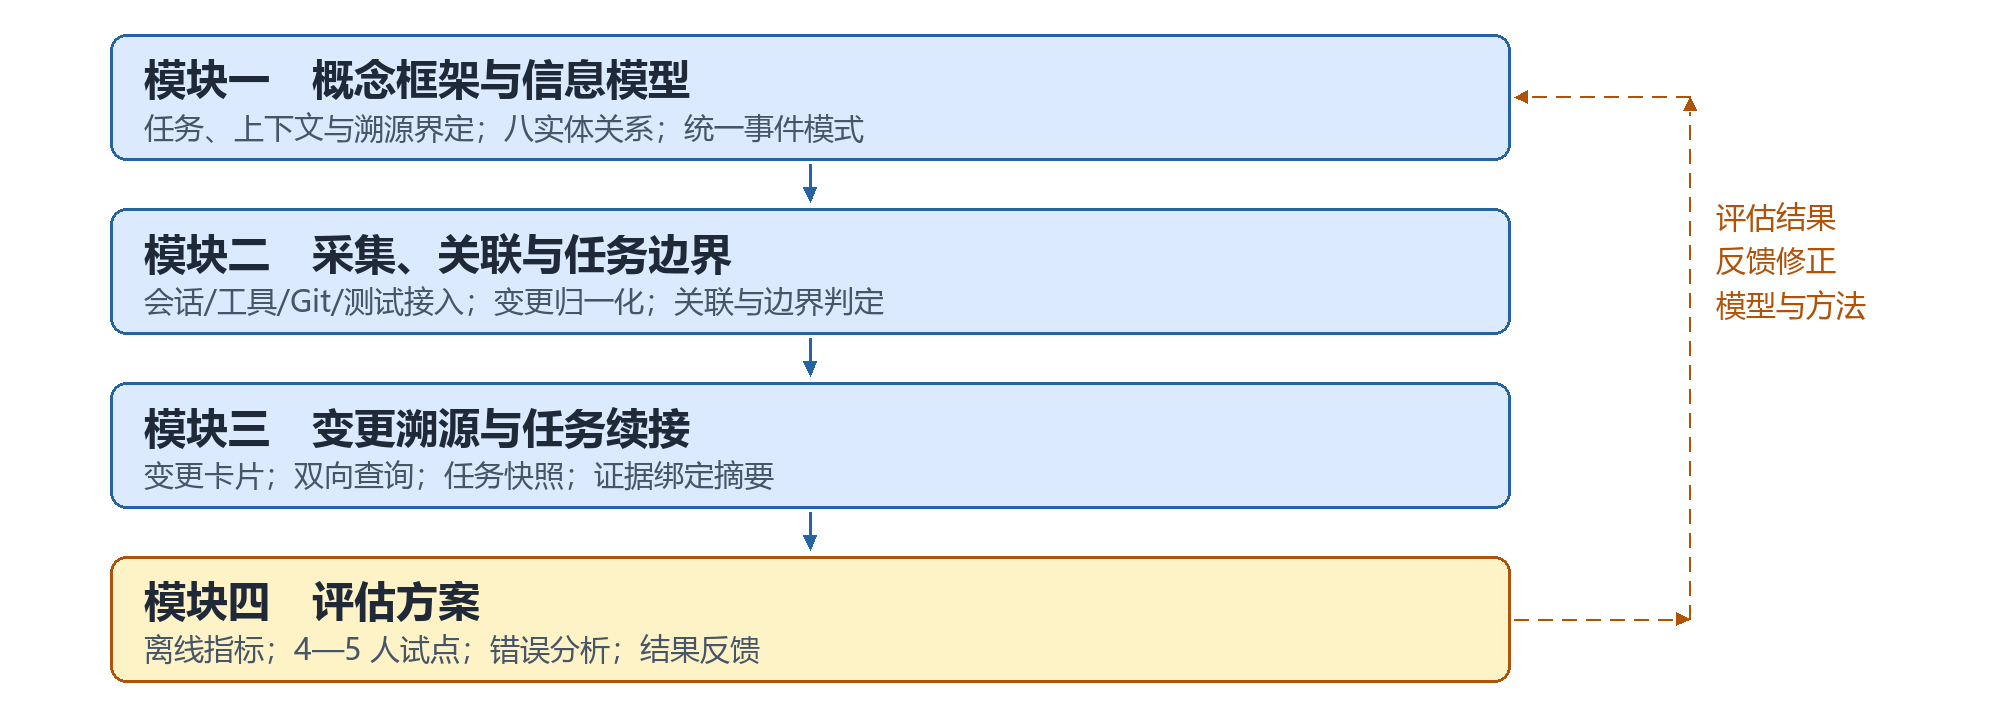
\includegraphics[width=\linewidth]{figures/fig1-route.png}
  \caption{研究技术路线}
  \label{fig:route}
\end{figure}

\tjformsubsub{（一）概念框架与信息模型}

本模块界定开发任务、任务上下文与变更溯源三个核心概念，并提出可计算的信息模型。开发任务指开发者发起的一次有明确目标的开发工作单元；任务上下文指与该任务相关的对话、变更、执行、测试、决策与未完成事项的集合；变更溯源指从一段代码变更出发，追溯其触发来源、实施过程、验证依据与后续演化的证据链。在此基础上，将任务上下文刻画为以任务为根的有向异构图：节点包括任务、对话轮次、消息、工具调用、文件变更（含变更块）、测试运行、测试用例结果与检查点，边包括包含、触发、产出、验证、演化与快照等关系，其基本结构如图~\ref{fig:model} 所示。以任务为根而非以会话或文件为根，是为了让跨会话、跨文件的记录围绕同一目标聚合，并为后续的边界判定与证据查询提供统一入口。该模型与 PROV-O[32] 的基本思想一致，但针对智能体事件流增加了任务边界、变更块与验证依据等约束。事件采用统一的 JSON 结构表示，字段涵盖标识、类型、时间、主体、来源、载荷与关联；模型需满足变更标识稳定、消息与变更多对多、测试结果双向指向等基本约束。上述概念与模型为后续采集、关联与查询提供共同语言，其具体表结构与索引方式将在原型实现阶段细化。

\begin{figure}[H]
  \centering
  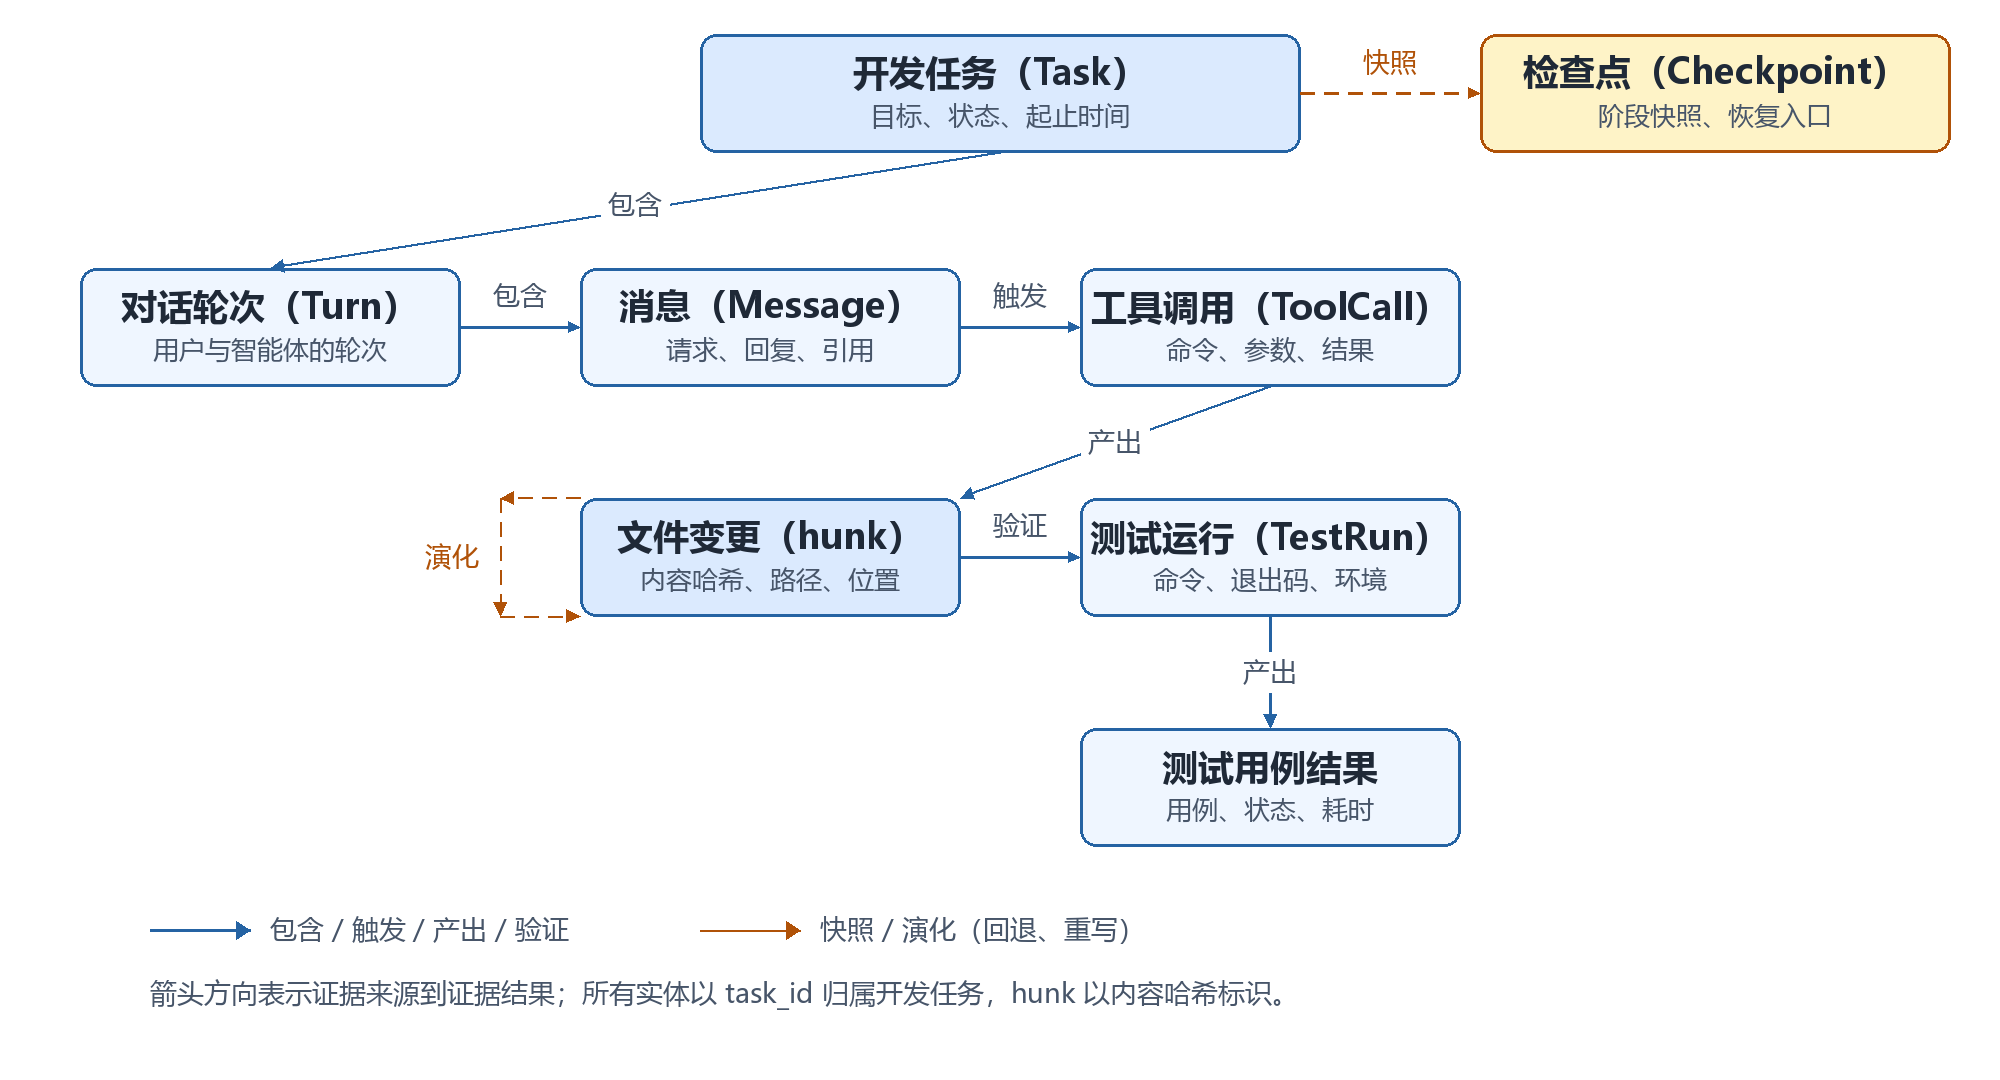
\includegraphics[width=\linewidth]{figures/fig2-model.png}
  \caption{任务上下文的信息模型}
  \label{fig:model}
\end{figure}

\tjformsubsub{（二）上下文采集、关联与任务边界}

本模块研究如何从真实开发过程中获得上述实体，并建立它们之间的关联。采集对象包括代码智能体的会话与工具调用、文件系统与 Git 变更、测试运行与结果；接入方式以 Claude Code 的官方钩子与 stream-json 为主，本地日志与 Git 作为补充。由于不同工具的编辑动作形式不一，需要将“旧串→新串”、补丁、整文件写入等统一归一化为变更块；语法感知的符号定位可借助 tree-sitter[41] 一类解析器完成。关联层面，拟综合利用时间邻近、显式引用（路径、符号、行号、命令、测试名）与文件级位置映射三类线索，为每条消息与每个变更块计算关联强度。由于同一变更可能由多轮消息共同促成，关联结果保留置信度与多对多关系，而不强行归并为单一来源。任务边界判定则依据空闲时长、显式指令、目标切换与提交动作等特征，采用可解释的规则打分，以便向开发者说明判定依据。该模块的重点不在于追求单点最优，而在于形成一套可复现、可解释的关联流程，其参数与阈值将在小规模验证集上调整并报告敏感性。

\tjformsubsub{（三）变更溯源与任务续接}

本模块将前两个模块的表示与关联转化为开发者可查询、可使用的证据链。对每个变更块生成变更卡片，记录触发消息、相关工具调用、修改前后快照、验证测试与后续演化；查询支持从代码到原因、从原因到代码两个方向。任务续接以任务快照为核心：快照由任务上下文图生成，将事项分为已完成、未完成与待验证三类，并附带指向证据的链接，使开发者能够从摘要直接跳转到对应的消息、变更或测试结果。原型拟采用 Web 形态，提供任务中心、任务时间线与变更证据侧栏三个视图；文件与代码片段视角作为时间线的过滤与详情，不单独作为第四视图。三个视图分别回答“当前有哪些任务”“任务经过了什么”“某处变更依据何在”，共同构成从任务到证据的浏览路径。大语言模型用于生成任务摘要与进展整理，但输出须绑定证据标识，证据不足时弃答，以降低无依据结论的风险。

\tjformsubsub{（四）评估方案}

本模块检验前三个模块的构想是否可行。研究定位为小样本探索性预研，不追求确证性结论。离线评测拟在 2 个中小规模开源仓库的 6—8 个任务上进行，任务覆盖缺陷修复、功能新增与代码重构，其中部分可改写自 SWE-bench 与 SWE-rebench[42] 的真实 issue；考察关联准确率、任务边界判定 F1、溯源查询正确率与查询响应时间等指标。用户研究拟招募 4—5 名具备编程经验的同专业学生，在自我中断情境下比较“Git 日志 + 原始会话记录”与“完整系统”两种条件，观察恢复用时、理解要点命中数与问题定位用时，并以 SUS[43] 作为可用性指标，NASA-TLX[44] 作为可选的认知负荷观察。受样本量限制，结果以描述统计与逐人差值呈现，不设显著性结论；同时通过任务构造与评测分离、第三方招募、数据脱敏等方式控制实验者偏差与伦理风险。离线指标用于检验方法的客观正确性，用户研究用于观察其在真实恢复情境中的可用性，二者互为补充。

四个模块的推进顺序为：先完成概念与模型、采集与关联的方法设计，再实现溯源与续接原型，最后开展评估，并将评估结果反馈至模型与方法。各模块的阶段性产出作为下一模块的输入，具体任务与周次见下文进度安排。

\clearpage
\tjformsubsection{3．工作进度安排}

本课题按任务书的教学周安排推进，六个阶段如表~\ref{tab:schedule} 与图~\ref{fig:gantt} 所示。第 9 周进行开题答辩，开题材料在第 8 周前完成；中期检查与答辩按学院统一安排。时间安排以教学周计，具体以学院通知为准。

\begin{table}[H]
  \centering
  \caption{研究进度安排}
  \label{tab:schedule}
  \begin{tabularx}{\linewidth}{@{}>{\raggedright\arraybackslash}p{3.2cm}>{\centering\arraybackslash}p{1.4cm}>{\raggedright\arraybackslash}X>{\raggedright\arraybackslash}p{3.2cm}@{}}
    \toprule
    阶段 & 教学周 & 主要工作 & 阶段成果 \\
    \midrule
    1　文献研究与产品调研 & 1—8 & 文献综述与竞品分析；确定研究问题、评价标准与实验任务；完成开题报告与答辩准备 & 文献综述、开题报告 \\
    2　关键方法设计与实现 & 9—14 & 信息模型与事件模式、编辑动作归一化、关联与边界判定、证据链查询 & 方法设计、实验脚本 \\
    3　系统设计与实现 & 15—20 & 三个视图、任务快照与续接、大模型摘要与证据校验、原型集成 & 原型 v0.9 \\
    4　系统验证与测试 & 21—22 & 6—8 个典型任务实验、4—5 人试点、错误分析与效度检查 & 实验数据、评估报告 \\
    5　毕业设计论文撰写 & 23—28 & 实验分析、论文初稿、图表与复现材料 & 论文初稿 \\
    6　论文审阅与修改 & 29—32 & 论文修改、查重、定稿与答辩材料 & 论文定稿、答辩材料 \\
    \bottomrule
  \end{tabularx}
\end{table}

\begin{figure}[H]
  \centering
  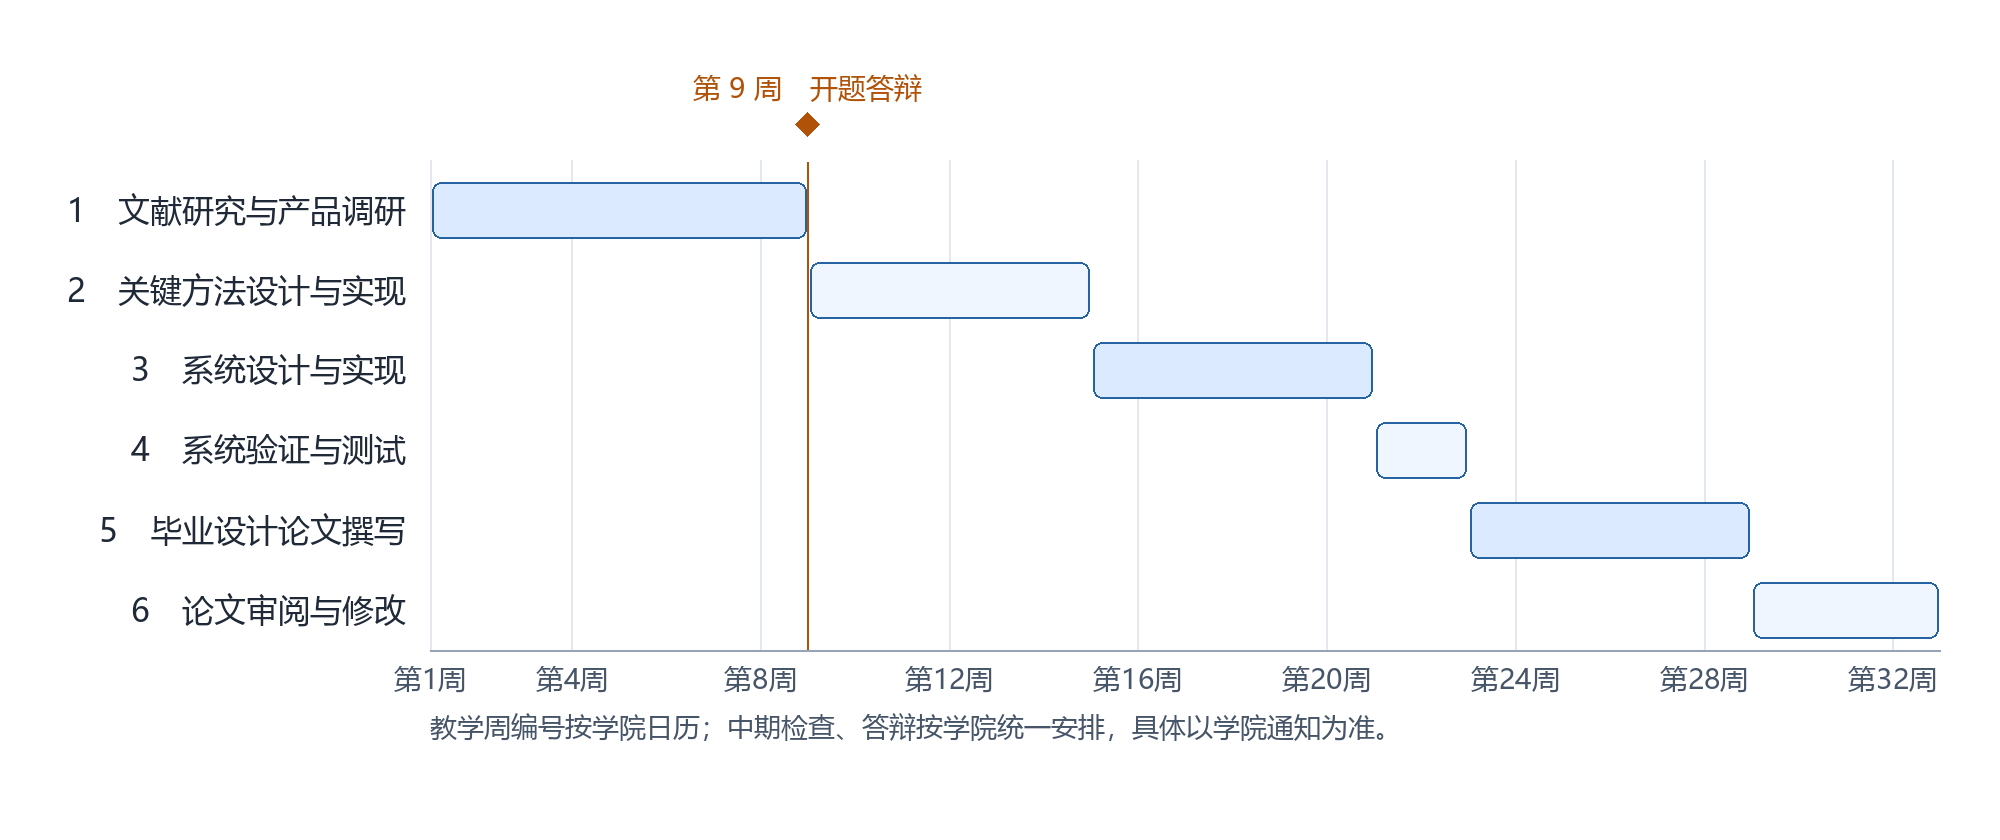
\includegraphics[width=\linewidth]{figures/fig3-gantt.png}
  \caption{研究进度甘特图}
  \label{fig:gantt}
\end{figure}

\clearpage
\tjformsection{三、\tjheadertext 的主要参考文献}\tjformsecnum{3}

（说明：会议文献按 GB/T 7714-2015 著录，出版地与出版者从略；网络资源引用日期统一为 2026-10-27。）

% 文献表按 Word 定稿：五号（10.5pt）、单倍行距；tjreflist 本身不设字号，故在此包一层。
{\zihao{5}\linespread{1}\selectfont\raggedright
\begin{tjreflist}
\item JIMENEZ C E, YANG J, WETTIG A, et al. SWE-bench: can language models resolve real-world GitHub issues?[C]//Proceedings of the 12th International Conference on Learning Representations. 2024. arXiv: 2310.06770.
\item CHEN M, TWOREK J, JUN H, et al. Evaluating large language models trained on code[EB/OL]. (2021-07-07)[2026-10-27]. https://arxiv.org/abs/2107.03374.
\item YANG J, JIMENEZ C E, WETTIG A, et al. SWE-agent: agent-computer interfaces enable automated software engineering[C]//Advances in Neural Information Processing Systems 37. 2024. arXiv: 2405.15793.
\item WANG X, LI B, SONG Y, et al. OpenHands: an open platform for AI software developers as generalist agents[C]//Proceedings of the 13th International Conference on Learning Representations. 2025. arXiv: 2407.16741.
\item WANG X, CHEN Y, YUAN L, et al. Executable code actions elicit better LLM agents[C]//Proceedings of the 41st International Conference on Machine Learning. 2024. arXiv: 2402.01030.
\item HONG S, ZHUGE M, CHEN J, et al. MetaGPT: meta programming for a multi-agent collaborative framework[C]//Proceedings of the 12th International Conference on Learning Representations. 2024. arXiv: 2308.00352.
\item QIAN C, LIU W, LIU H, et al. ChatDev: communicative agents for software development[C]//Proceedings of the 62nd Annual Meeting of the Association for Computational Linguistics. 2024: 15174-15186. DOI: 10.18653/v1/2024.acl-long.810.
\item XIA C S, DENG Y, DUNN S, et al. Agentless: demystifying LLM-based software engineering agents[EB/OL]. (2024-07-01)[2026-10-27]. https://arxiv.org/abs/2407.01489.
\item HOU X, ZHAO Y, LIU Y, et al. Large language models for software engineering: a systematic literature review[J]. ACM Transactions on Software Engineering and Methodology, 2024, 33(8). DOI: 10.1145/3695988.
\item FAN A, GOKKAYA B, HARMAN M, et al. Large language models for software engineering: survey and open problems[EB/OL]. (2023-10-05)[2026-10-27]. https://arxiv.org/abs/2310.03533.
\item 张犬俊, 谢杨, 房春荣, 等. 检索增强生成在软件工程中的应用综述[J]. 软件学报, 2026, 37(3): 1316-1339. DOI: 10.13328/j.cnki.jos.007567.
\item 汪莹, 字千成, 彭鑫, 等. 基于大语言模型的故障复现测试用例生成方法[J]. 软件学报, 2026, 37(4): 1690-1714. DOI: 10.13328/j.cnki.jos.007474.
\item PENG S, KALLIAMVAKOU E, CIHON P, et al. The impact of AI on developer productivity: evidence from GitHub Copilot[EB/OL]. (2023-02-13)[2026-10-27]. https://arxiv.org/abs/2302.06590.
\item MOZANNAR H, BANSAL G, FOURNEY A, et al. Reading between the lines: modeling user behavior and costs in AI-assisted programming[C]//Proceedings of the CHI Conference on Human Factors in Computing Systems. 2024: 1-16. DOI: 10.1145/3613904.3641936.
\item PERRY N, SRIVASTAVA M, KUMAR D, et al. Do users write more insecure code with AI assistants?[C]//Proceedings of the 2023 ACM SIGSAC Conference on Computer and Communications Security. 2023: 2785-2799. DOI: 10.1145/3576915.3623157.
\item BARKE S, JAMES M B, POLIKARPOVA N. Grounded Copilot: how programmers interact with code-generating models[J]. Proceedings of the ACM on Programming Languages, 2023, 7(OOPSLA1): 85-111. DOI: 10.1145/3586030.
\item VAITHILINGAM P, ZHANG T, GLASSMAN E L. Expectation vs. experience: evaluating the usability of code generation tools powered by large language models[C]//Proceedings of the CHI Conference on Human Factors in Computing Systems Extended Abstracts. 2022: 1-7. DOI: 10.1145/3491101.3519665.
\item ŚLIWERSKI J, ZIMMERMANN T, ZELLER A. When do changes induce fixes?[C]//Proceedings of the 2005 International Workshop on Mining Software Repositories. 2005: 1-5. DOI: 10.1145/1083142.1083147.
\item KAGDI H, COLLARD M L, MALETIC J I. A survey and taxonomy of approaches for mining software repositories in the context of software evolution[J]. Journal of Software Maintenance and Evolution: Research and Practice, 2007, 19(2): 77-131. DOI: 10.1002/smr.344.
\item ROBBES R, LANZA M. A change-based approach to software evolution[J]. Electronic Notes in Theoretical Computer Science, 2007, 166: 93-109. DOI: 10.1016/j.entcs.2006.06.015.
\item FALLERI J R, MORANDAT F, BLANC X, et al. Fine-grained and accurate source code differencing[C]//Proceedings of the 29th ACM/IEEE International Conference on Automated Software Engineering. 2014: 313-324. DOI: 10.1145/2642937.2642982.
\item GRUND F, CHOWDHURY S A, BRADLEY N C, et al. CodeShovel: constructing method-level source code histories[C]//Proceedings of the 43rd International Conference on Software Engineering. 2021: 1510-1522. DOI: 10.1109/ICSE43902.2021.00135.
\item KERSTEN M, MURPHY G C. Using task context to improve programmer productivity[C]//Proceedings of the 14th ACM SIGSOFT International Symposium on Foundations of Software Engineering. 2006: 1-11. DOI: 10.1145/1181775.1181777.
\item DRAGUNOV A N, DIETTERICH T G, JOHNSRUDE K, et al. TaskTracer: a desktop environment to support multi-tasking knowledge workers[C]//Proceedings of the 10th International Conference on Intelligent User Interfaces. 2005: 75-82. DOI: 10.1145/1040830.1040855.
\item BAO L, YE D, XING Z, et al. ActivitySpace: a remembrance framework to support interapplication information needs[C]//Proceedings of the 30th IEEE/ACM International Conference on Automated Software Engineering. 2015: 864-869. DOI: 10.1109/ASE.2015.90.
\item BEGEL A, KHOO Y P, ZIMMERMANN T. Codebook: discovering and exploiting relationships in software repositories[C]//Proceedings of the 32nd ACM/IEEE International Conference on Software Engineering. 2010: 125-134. DOI: 10.1145/1806799.1806821.
\item PARNIN C, RUGABER S. Resumption strategies for interrupted programming tasks[J]. Software Quality Journal, 2011, 19(1): 5-34. DOI: 10.1007/s11219-010-9104-9.
\item PARNIN C, DELINE R. Evaluating cues for resuming interrupted programming tasks[C]//Proceedings of the SIGCHI Conference on Human Factors in Computing Systems. 2010: 93-102. DOI: 10.1145/1753326.1753342.
\item SAFER I, MURPHY G C. Comparing episodic and semantic interfaces for task boundary identification[C]//Proceedings of the 2007 Conference of the Center for Advanced Studies on Collaborative Research. 2007: 229-243. DOI: 10.1145/1321211.1321235.
\item ROBBES R, LANZA M. Characterizing and understanding development sessions[C]//Proceedings of the 15th IEEE International Conference on Program Comprehension. 2007: 155-166. DOI: 10.1109/ICPC.2007.12.
\item CHENEY J, CHITICARIU L, TAN W C. Provenance in databases: why, how, and where[J]. Foundations and Trends in Databases, 2009, 1(4): 379-474. DOI: 10.1561/1900000006.
\item W3C. PROV-O: the PROV ontology[EB/OL]. (2013-04-30)[2026-10-27]. https://www.w3.org/TR/prov-o/.
\item SOUZA R, GUEROUDJI A, DEWITT S, et al. PROV-AGENT: unified provenance for tracking AI agent interactions in agentic workflows[C]//Proceedings of the 21st IEEE International Conference on e-Science. 2025. arXiv: 2508.02866.
\item KO A J, MYERS B A. Designing the Whyline: a debugging interface for asking questions about program behavior[C]//Proceedings of the SIGCHI Conference on Human Factors in Computing Systems. 2004: 151-158. DOI: 10.1145/985692.985712.
\item PIMENTEL J F, MURTA L, BRAGANHOLO V, et al. noWorkflow: a tool for collecting, analyzing, and managing provenance from Python scripts[J]. Proceedings of the VLDB Endowment, 2017, 10(12): 1841-1844. DOI: 10.14778/3137765.3137789.
\item Anthropic. Claude Code documentation: overview[EB/OL]. [2026-10-27]. https://code.claude.com/docs/en/overview.
\item Cursor. Cursor documentation[EB/OL]. [2026-10-27]. https://cursor.com/docs.
\item Cline. Cline: AI coding, open source and open choice[EB/OL]. [2026-10-27]. https://cline.bot.
\item Langfuse. Observability overview[EB/OL]. [2026-10-27]. https://langfuse.com/docs/observability/overview.
\item OpenTelemetry. Generative AI semantic conventions[EB/OL]. [2026-10-27]. https://github.com/open-telemetry/semantic-conventions-genai.
\item Tree-sitter. Tree-sitter documentation[EB/OL]. [2026-10-27]. https://tree-sitter.github.io/tree-sitter/.
\item BADERDINOV I, GOLUBEV A, NEKRASHEVICH M, et al. SWE-rebench: an automated pipeline for task collection and decontaminated evaluation of software engineering agents[EB/OL]. (2025-05-26)[2026-10-27]. https://arxiv.org/abs/2505.20411.
\item BROOKE J. SUS: a quick and dirty usability scale[M]//JORDAN P W, THOMAS B, WEERDMEESTER B A, et al. Usability Evaluation in Industry. London: Taylor \& Francis, 1996: 189-194.
\item HART S G, STAVELAND L E. Development of NASA-TLX (Task Load Index): results of empirical and theoretical research[J]. Advances in Psychology, 1988, 52: 139-183. DOI: 10.1016/S0166-4115(08)62386-9.
\end{tjreflist}
}

% 审核意见单独起页：两个意见框与“四、”标题合计超过一页余量，
% 不分页会把“专业审核意见”框挤到下一页，与 Word 版（审核意见独占末页）不一致。
\newpage
\tjformsection{四、审核意见}\tjformsecnum{4}

\begin{tjreviewbox}
  \tjformlabel{指导教师意见：}\tjformhint{（课题难度是否适中、工作量是否饱满、进度安排是否合理、工作条件是否具备、是否同意开题等）}

  \vspace{8\baselineskip}
  \tjformsignature{指导教师签名}{8em}
\end{tjreviewbox}

\begin{tjreviewbox}
  \tjformlabel{专业审核意见：}\tjformhint{（适当对各项内容给与意见和评价，字数不限。）}

  \vspace{6\baselineskip}
  \tjformsignature{负责人签名}{8em}
\end{tjreviewbox}
